\section{Data Models and Validation}

A data model is an abstract view over the data that hides the way it is stored physically. When going from the physical view (Syntax) to the logical view (Data Model) we speak about parsing and vice versa about serializing.

\subsection{The JSON Information Set}

The appropriate abstraction for any JSON document is a tree. The nodes of that tree, which are JSON logical values, are naturally of six possible kinds: the six syntactic building blocks of JSON. These are the four leaves corresponding to atomic values: Strings, Numbers, Booleans and Nulls. As well as two intermediate nodes (possibly leaves if empty): Objects (String-to-value map) and Arrays (List of values).

Formally, and not only for JSON but for all tree-based models, these nodes are generally called \textit{information items} and form the logical building blocks of the model, called \textit{information set}.

When a JSON document is being parsed by a JSON library, this tree is built in memory, the edges being pointers, and further processing will be done on the tree and not on the original syntax.

\subsection{The XML Information Set}

It is possible to do the same logical abstraction, also based on trees, with XML, where information items correspond to elements, attributes, text, etc.

A fundamental difference between JSON trees and XML trees is that for JSON, the labels (object keys) are on the edges connecting an object information item to each one of its children information items. In XML, the labels (these would be element and attribute names) are on the nodes (information items) directly. Another way to say it is that a JSON information item does not know with which key it is associated in an object (if at all), while an XML element or attribute information item knows its name.

\begin{figure}[h]
    \centering
    \begin{subfigure}{0.495\textwidth}
        \centering
        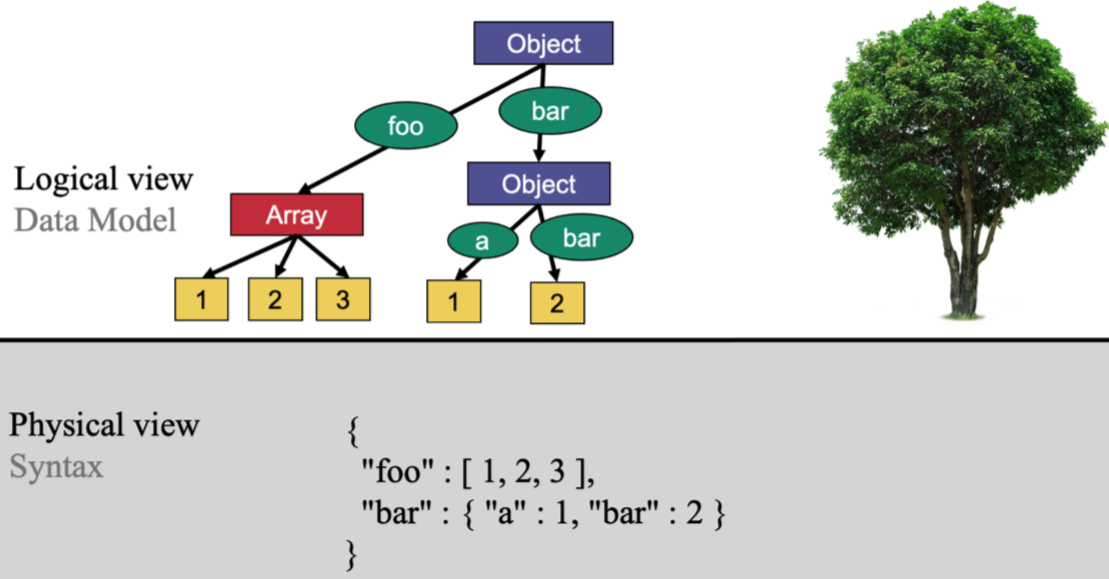
\includegraphics[width=\textwidth]{Figures/JSONTree.jpeg}
        \caption{JSON Tree}\label{subfig:JSONTree}
    \end{subfigure}
    \hfill
    \begin{subfigure}{0.495\textwidth}
        \centering
        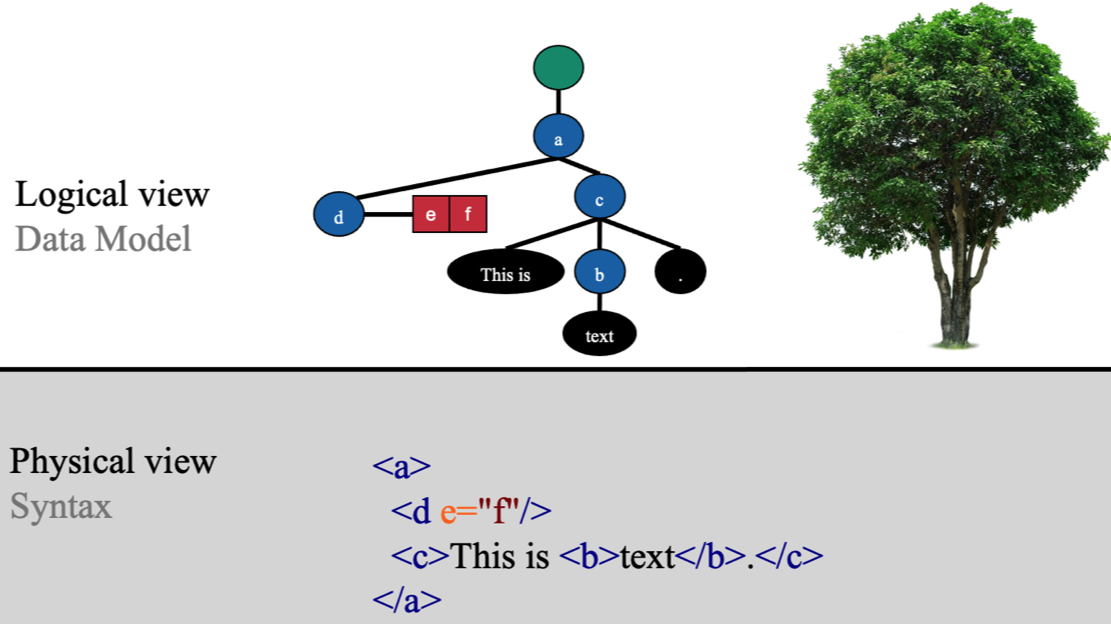
\includegraphics[width=\textwidth]{Figures/XMLTree.jpeg}
        \caption{XML Tree}\label{subfig:XMLTree}
    \end{subfigure}
    \caption{Tree Structures}\label{fig:Trees}
\end{figure}

There are many information items in XML. Here, we will focus on documents, elements, attributes and characters and discuss these based on the following example:

\begin{figure}[h]
    \centering
    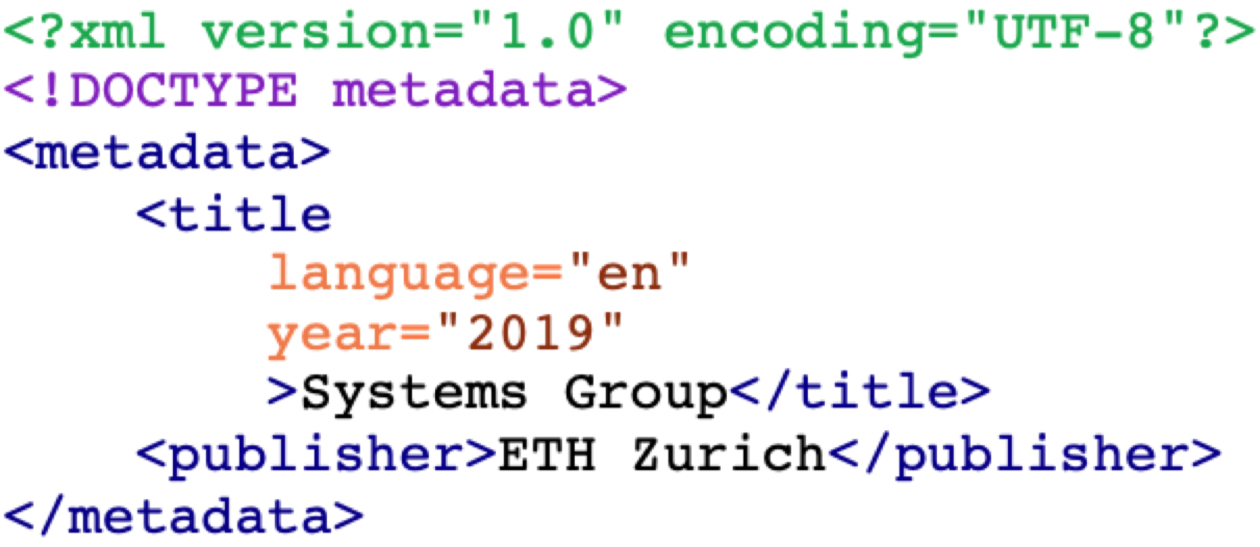
\includegraphics[width=0.6\textwidth]{Figures/XMLexplCode.jpeg}
    \caption{Example XML Document}\label{fig:XMLexpl}
\end{figure}

\subsubsection{Document Information Item}
The document information item is just the root of an XML tree. It does not correspond to anything syntactically or, if at all, it would correspond to the text and doctype declarations. In the example in \cref{fig:XMLexpl}, the documentation information has two important properties:
\begin{itemize}
    \item $\eckigeklammer{\text{children}}$ Element information item \textit{metadata}
    \item $\eckigeklammer{\text{version}}$ 1.0
\end{itemize}

\subsubsection{Element Information Item}
There is one element information item for each element. Here we have three.
The element information item \textit{metadata} has four important properties:
\begin{itemize}
    \item $\eckigeklammer{\text{local name}}$ metadata
    \item $\eckigeklammer{\text{children}}$ Element Information Item \textit{title}, Element Information Item \textit{publisher}
    \item $\eckigeklammer{\text{attribute}}$ (empty)
    \item $\eckigeklammer{\text{parent}}$ Document Information Item
\end{itemize}
The element information item \textit{title} has four important properties:
\begin{itemize}
    \item $\eckigeklammer{\text{local name}}$ title
    \item $\eckigeklammer{\text{children}}$ Character Information Item \textit{Systems Group}
    \item $\eckigeklammer{\text{attributes}}$ Attribute Information Item \textit{language}, Attribute Information Item \textit{year}
    \item $\eckigeklammer{\text{parent}}$ Element Information Item \textit{metadata}
\end{itemize}
The element information item \textit{publisher} has four important properties:
\begin{itemize}
    \item $\eckigeklammer{\text{local name}}$ publisher
    \item $\eckigeklammer{\text{children}}$ Character Information Item \textit{ETH Zurich}
    \item $\eckigeklammer{\text{attribute}}$ (empty)
    \item $\eckigeklammer{\text{parent}}$ Element Information Item \textit{metadata}
\end{itemize}

\subsubsection{Attribute Information Item}
There is one attribute information item for each attribute. Here we have two.
The attribute information item \textit{language} has three important properties:
\begin{itemize}
    \item $\eckigeklammer{\text{local name}}$ language
    \item $\eckigeklammer{\text{normalized value}}$ en
    \item $\eckigeklammer{\text{owner element}}$ Element Information Item \textit{title}
\end{itemize}
The attribute information item \textit{year} has three important properties:
\begin{itemize}
    \item $\eckigeklammer{\text{local name}}$ year
    \item $\eckigeklammer{\text{normalized value}}$ 2019
    \item $\eckigeklammer{\text{owner element}}$ Element Information Item \textit{title}
\end{itemize}

\subsubsection{Character and Text Information Item}
There are as many character information items as characters in text (between tags). For example, for the S in Systems Group:
\begin{itemize}
    \item $\eckigeklammer{\text{character code}}$ the unicode code point for the letter S
    \item $\eckigeklammer{\text{parent}}$ Element Information Item \textit{title}
\end{itemize}
It is sometimes simpler to group them into a single (non standard) text information item:
\begin{itemize}
    \item $\eckigeklammer{\text{characters}}$ S y s t e m s $<$space$>$ G r o u p
    \item $\eckigeklammer{\text{parent}}$ Element Information Item \textit{title}
\end{itemize}

\subsubsection{The entire tree}
All information items built previously can finally be assembled and drawn as a tree. The edges, corresponding to children and parent (or owner element) properties, will correspond to pointers in memory when the tree is built by the XML library:

\begin{figure}[h]
    \centering
    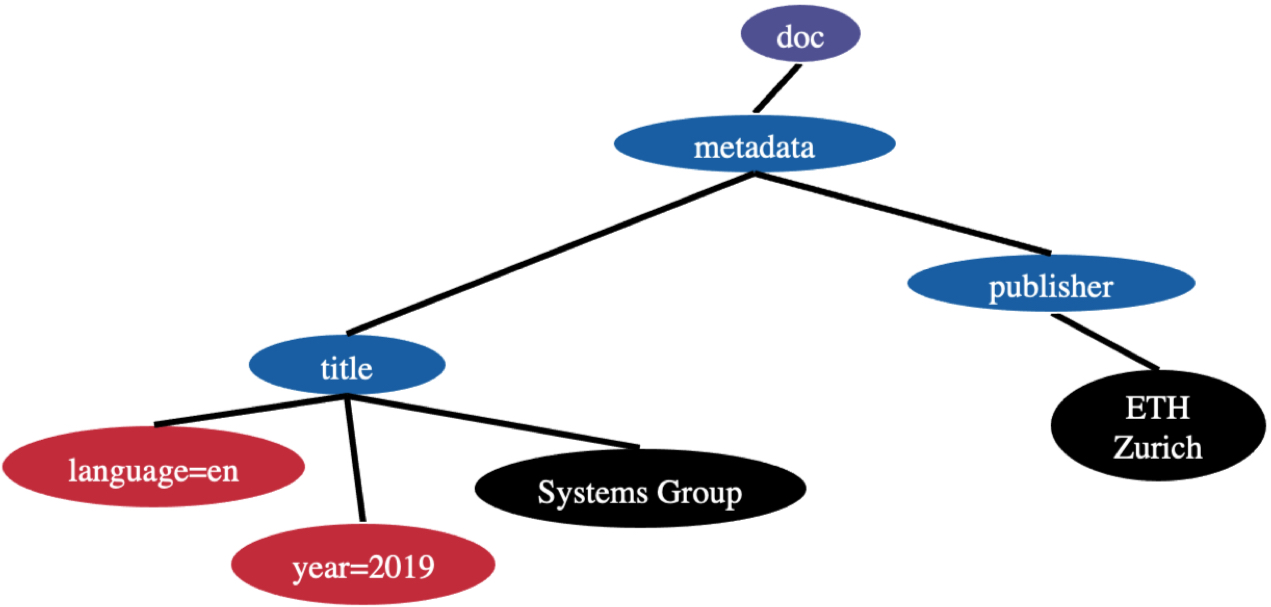
\includegraphics[width=0.5\textwidth]{Figures/XMLTree2.jpeg}
    \caption{Assembled XML Tree.}\label{fig:XMLTree2}
\end{figure}

\subsection{Validation}
Validation is not the same as well-formedness.
Once documents, JSON or XML, have been parsed and logically abstracted as a tree in memory, the natural next step is to check for further structural constraints.

For example, you could want to check whether your JSON documents all associate key “name” with a string, or if they all associate “years” with an array of positive integers. Or you could want to check whether your XML documents all have root elements called “persons,” and whether the root element in each document has only children elements called “person,” all with an attribute “first” and an attribute “last.”

This might remind the reader of schemas in a relational database, but with a major difference: in a relational database, the schema of a table is defined before any data is populated into the table. Thus, the data in the table is guaranteed, at all times, to fulfil all the constraints of the schema. The exact term is that the data is guaranteed to be valid against the schema, because the schema was enforced at write time (schema on write).

But in the case of a collection of JSON and XML documents, this is the other way round. A collection of JSON and XML documents out there can exist without any schema and contain arbitrary structures. Validation happens “ex post,” that is, only after reading the data (schema on read).

Thus, it means that JSON and XML documents undergo two steps:
\begin{itemize}
    \item a well-formedness check: attempt to parse the document and consruct a tree representation in memory
    \item (if the first step succeeded) a validation check given a specific schema
\end{itemize}
Validation is schema dependent: a given well-formed document can be valid against schema A and invalid against schema B.

Validation is often performed on much more than a document at a time: an entire collection. Thus, we distinguish between heterogeneous collections, whose documents are not valid against any particular schema, and homogeneous collections, whose documents are all valid against a specific schema.

\subsection{Item Types}
A fundamental aspect of validation is the type system. A well-designed type system, in turn, allows for storing the data in much more efficient, binary formats tailored to the model.

The first aspect that almost all, if not all type systems, have in common, is the distinction between atomic types and structured types.

\subsubsection{Atomic Types}
Atomic types correspond to the leaf of a tree data model: these are types that do not contain any further nestedness.

\subsubsection*{Strings}
Strings are simply finite sequences of (usually printable) characters. Formally, strings form a monoid under concatenation, where the neutral element is the empty string.

All atomic types have in common that they have a logical value space and a lexical value space. The logical value space corresponds to the actual logical abstraction of the type (e.g., a mathematical set of integers), while the lexical value space corresponds to the representation of logical values in a textual format (such as the decimal, or binary, or hexadecimal representation of an integer).

Often, the lexical representation of a string is double-quoted, sometimes also single-quoted.

The difference between the lexical representation and the logical value of a string becomes immediately apparent when escaping is used. For example, the lexical representation "$\backslash \backslash \backslash$" corresponds to the (logical) string "$\backslash$".

\subsubsection*{Numbers}

\paragraph{Integers}
In older programming languages, support for integers used to be bounded. This is why classical types, still in use today, correspond to 8-bit (often called byte), 16-bit (often called short), 32-bit (often called int) and 64-bit integers (often called long). This means that, expressed in base 2, they use 8, 16, 32 or 64 bits (binary digits).
However, in modern databases, it is customary to support unbounded integers.

The lexical representation of integers is usually done is base 10, in the familiar decimal system, even though base 2, 8 or 16 can be found, too. Leading 0s are optional, but when an logical integer value is canonically serialized, it is done without a leading 0.

\paragraph{Decimals}
Decimals correspond to real numbers that can be written as a finite sequence of digits in base 10, with an optional decimal period. Equivalently, these are fractions that can be expressed with a power of 10 in the denominator.
Many modern databases or storage formats support the entire logical decimal value space with no restriction on how large, small or precise a decimal number is.

The number of digits in the whole decimal number is called the precision and the number of digits behind the comma is called the scale.

\paragraph{Floating-Point}
Floating-point numbers are limited both in precision and magnitude (both upper and lower) in order to fit on 32 bits (float) or 64 bits (double). Floats have about 7 digits of precision and their absolute value can be between roughly $10^{-37}$ and $10^{37}$, while doubles have 15 digits of precision and their absolute value can be between roughly $10^{-307}$ and $10^{308}$.

Double and float types also cover additional special values: NaN (not a number), positive and negative infinity, and negative zero (in addition to the “positive” 0).

The lexical representation of floats and doubles often use the scientific notation: \texttt{-12.34E-56}.
And the lexical values corresponding to the special logical values look like so: \texttt{NaN}, \texttt{INF}, \texttt{-INF}, \texttt{-0}.


\paragraph{Booleans}
The logical value space for the Boolean type is made of two values: true and false as in NoSQL queries, two-valued logic is typically assumed.
The corresponding lexical values are typically \texttt{true} and \texttt{false}.

\paragraph{Dates and Times}
Dates are commonly using the Gregorian calendar with a year (BC or AD), a month and a day of the month. Dates require quotes!

Times are expressed in the hexagesimal (60) basis with hours, minutes, seconds, where the seconds commonly go all the way to microseconds (six digits after the decimal period).

Datetimes are expressed with a year, a month, a day of the month, hours, minutes and (decimal) seconds.

The timestamp type corresponds to a datetime with a timezone, but treating datetimes as equivalent if they express the same point in time. Timestamp values are typically stored as longs (64-bit integers) expressing the number of milliseconds elapsed since January 1, 1970 by convention.

The lexical values can also vary, although many technologies follow the ISO 8601 standard, where lexical values look like so (with many parts optional): \texttt{2022-08-07T14:18:00.123456+02:00}, \texttt{2022-08-07}, \texttt{14:18:00.123456}, \texttt{14:18:00.123456Z}.

\paragraph{Durations}
Durations can be of many different kinds, generally a combination of years, months, days, hours, minutes and (possibly with decimals) seconds.
What is important to understand is that there is a “wall” between months and days: what is the duration “1 month and 1 day?” It could be 29, 30, 31, or 32 days and should thus be avoided. Thus, most durations, for the sake of being unambiguous, are either involving years and/or months, or are involving days and/or hours and/or minutes and/or seconds.

The lexical representation can vary, but there is a standard defined by ISO 8601 as well, starting with a P and prefixing sub-day parts with a T. Here some examples:
\begin{itemize}
    \item 2 years and 3 months: \texttt{P2Y3M}
    \item 4 days, 3 hours, 2 minutes and 1.123456 seconds: \texttt{P4DT3H2M1.123456}
    \item 3 hours, 2 minutes and 1.123456 seconds: \texttt{PT3H2M1.123456}
\end{itemize}

\paragraph{Binary Data}
Binary data is, logically, simply a sequence of bytes. There are two main lexical representations used in data: hexadecimal and base64. Hexadecimal expresses the data with two hexadecimal digits per byte, like so: \texttt{0123456789ABCDEF} which would correspond to the bit sequence:

\texttt{0000000100100011010001010110011110001001101010111100110111101111}.

\paragraph{Null}
Many technologies and formats also provide support for null values, although how this is done largely varies. Some technologies allow null to appear as a (valid) value for any type. A schema can either allow, or disallow the null value. Often, the terminology used is that a type can be nullable (or nillable) or not. Other technologies consider that there is a singleton-valued null type, containing only the null value with the lexical representation \texttt{null}.

Allowing nulls is done by taking the union of the desired type with the null type. Yet other technologies consider null when it appears as a value in an object to be semantically equivalent by the absence of a value and then, allowing or disallowing null is achieved by (e.g. in JSON) making the field required or optional. It is important to understand that the latter technologies are unable to distinguish between the following two JSON objects, so that information in the input dataset is lost upon validating:

\begin{lstlisting}[style=json, label={lst:jsonnull}]
{}
{ "foo" : null }
\end{lstlisting}

This can be problematic with datasets where this distinction is semantically relevant. XML also supports null values, but calls them “nil” and does so with a special attribute and no content rather than with a lexical representation

\begin{lstlisting}[style=xml, label={lst:xmlnull}]
<foo
    xmlns:xsi="http://www.w3.org/2001/XMLSchema-instance"
    xsi:nil="true"/>
\end{lstlisting}

\subsubsection{Structured Types}
The two main types are:
\begin{itemize}
    \item Lists. E.g. JSON Array, XML Element, DataFrame Array.
    \item Maps. E.g. JSON Object, Set of XML Attributes, DataFrame Struct.
\end{itemize}

\paragraph{Type Names}
Below there is a summary of many types over various technologies and languages and how they correspond to each other. The most important thing to see here is that on the high level, atomic types are almost always the same everywhere, even though the names can vary.

\begin{figure}[h]
    \centering
    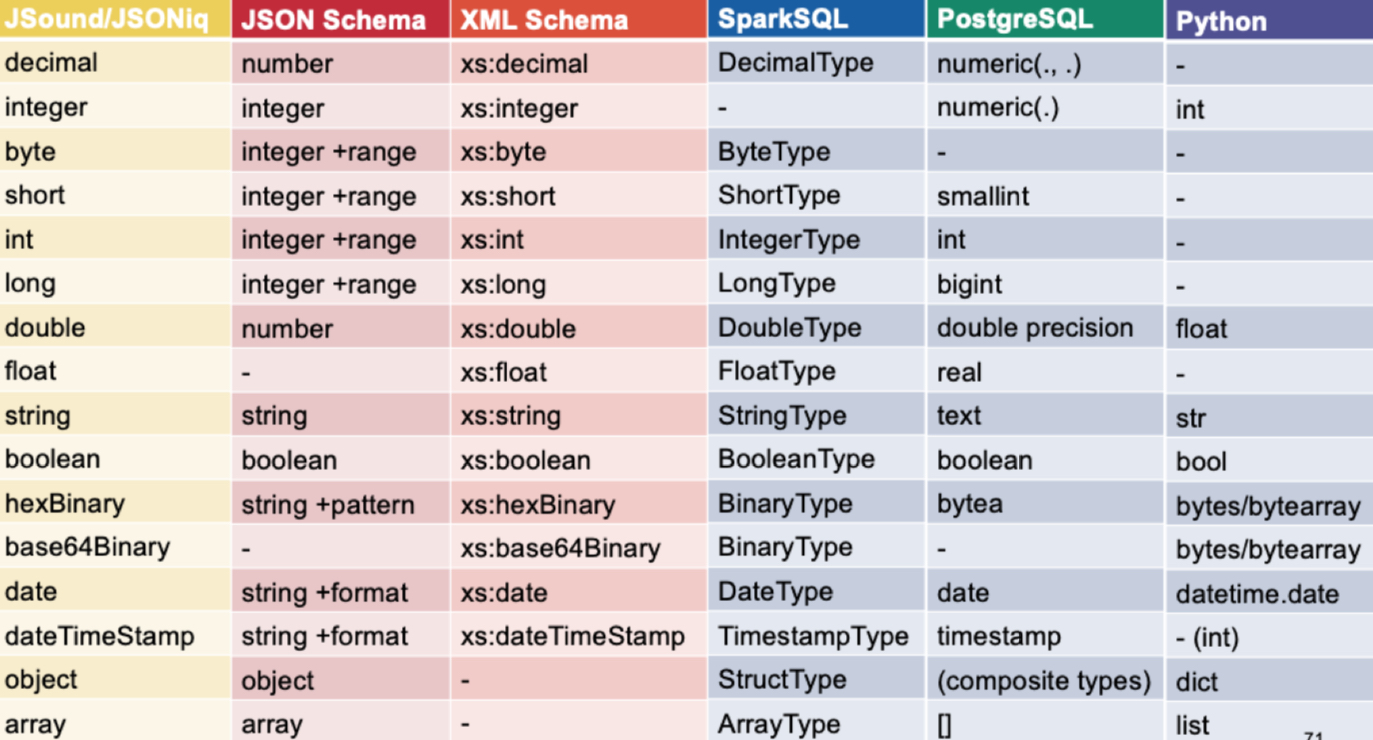
\includegraphics[width=0.9\textwidth]{Figures/TypeNames.jpeg}
    \caption{Type Names}\label{fig:TypeNames}
\end{figure}


\subsection{Sequence Types}

\paragraph{Cardinality}
In the context of data querying but also of nested lists and arrays, items (single values) rarely appear alone. They often appear as a sequence of many values. Thus, many type system give options regarding the number of occurrences of items in a sequence. There are four main occurrence indicators:
\begin{itemize}
    \item ust once (often implicit): exactly one item. Common adjective: required
    \item optional: zero or one item. Often represented witha question mark (?). Common adjective: optional
    \item any occurence: zero, one or more items. Often represented with a Kleen star (*). Common adjective: repeated
    \item at least once: one or more items. Often represented with a Kleene plus (+).
\end{itemize}

\subsection{JSON Validation / JSOUND}

\subsubsection{Validating flat objects}
A JSound-schema pair may look like this:

\begin{minipage}{0.45\textwidth}
\begin{lstlisting}[style=json,caption={JSON Code}]
{
    "name" : "Einstein",
    "first" : "Albert",
    "age" : 142
}
\end{lstlisting}
\end{minipage}
\hfill
\begin{minipage}{0.45\textwidth}
\begin{lstlisting}[style=json,caption={JSOUND Schema}]
{
    "name" : "string",
    "first" : "string",
    "age" : "integer"
}
\end{lstlisting}
\end{minipage}
“string” can be replaced with any other named type, in particular taken from the table shown in the former section. Let us list them here:
\begin{itemize}
    \item Strings: string, anyURI (for strings containing a URI);
    \item Numbers: decimal, integer, float, double, long, int, short, byte, negativeInteger, positiveInteger, nonNegativeInteger, nonPositiveInteger, unsignedByte, unsighedShort, unsignedInt, unsignedLong;
    \item Dates and times: date, time, dateTime, gYearMonth, gYear, gMonth, gDay, gMonthDay, dateTimeStamp;
    \item Time intervals: duration, yearMonthDuration, dayTimeDuration;
    \item Binary types: hexBinary, base64Binary
    \item Booleans: boolean
    \item Nulls: null
\end{itemize}
Alternatively to JSound, one can use JSON Schema for validation. The JSON Schema for the above JSON code is
\begin{lstlisting}[style=json,caption={Schema}]
{
    "type" : "object",
    "properties" : {
        "name" : "string",
        "first" : "string",
        "age" : "number"
    }
}
\end{lstlisting}
The available JSON Schema types are string, number, integer, boolean, null, array and object. This closely matches the original JSON syntax with the only exception that numbers have this additional integer subtype. The type system of JSON Schema is thus less rich than that of JSound, but extra checks can be done with so-called formats, which include date, time, duration, email, and so on including generic regular expressions. Like JSound, JSON Schema also allow restricting the length of a string, constraining numbers to intervals, etc.

\subsubsection{Requiring the presence of a key}
By default, the presence of a key is optional, so that each one of the following objects is also valid against the previous schema:
\begin{lstlisting}[style=json]
{ "name" : "Einstein" }
{ "first" : "Albert" }
{ "age" : 142 }
{ "name" : "Einstein", "age" : 142 }
{}
\end{lstlisting}
It is possible to require the presence of a key by adding an exclamation mark, like so.
\begin{lstlisting}[style=json]
{
"!name" : "string",
"!first" : "string",
"age" : "integer"
}
\end{lstlisting}
This is the equivalent JSON Schema, which uses a “required” property associated with the list of required keys to express the same:
\begin{lstlisting}[style=json]
{
    "type" : "object",
    "required" : [ "name", "first" ]
    "properties" : {
        "name" : "string",
        "first" : "string",
        "age" : "number"
    }
}
\end{lstlisting}

\subsubsection{Open and closed object types}
In the JSound compact syntax, extra keys are forbidden. The schema is said to be closed. There are ways to define JSound schemas to allow arbitrary additional keys (open schemas), with a more verbose syntax. Unlike JSound, in JSON Schema, extra properties are allowed by default. JSON Schema then allows to forbid extra properties with the “additionalProperties” property, like so:
\begin{lstlisting}[style=json]
{
    "type" : "object",
    "required" : [ "name", "first" ]
    "properties" : {
        "name" : "string",
        "first" : "string",
        "age" : "number"
    },
    "additionalProperties" : false
}
\end{lstlisting}

\subsubsection{Nested Structures}
Examples of nested schemas:
\begin{lstlisting}[style=json]
{ "numbers" : [ "integer" ] }
\end{lstlisting}
\begin{lstlisting}[style=json]
{ "matrix" : [ [ "decimal" ] ] }
\end{lstlisting}
Examples of valid JSON code for these two schemas:
\begin{lstlisting}[style=json]
{
    "numbers" : [ 1, 2, 6, 2, 7, 1, 57, 4 ]
}
\end{lstlisting}
\begin{lstlisting}[style=json]
{ "matrix" : [ [ 0, 1 ], [ 1, 0 ] ] }
\end{lstlisting}

With the JSound compact syntax, object and array types can nest arbitrarily:
\begin{lstlisting}[style=json]
{
    "datapoints" : [
        {
            "features" : [ "double" ],
            "label" : "integer"
        }
    ]
}
\end{lstlisting}

\vspace{1\baselineskip}

Every schema can be given a name, turning into a type. When a document is valid against a schema, it is typical to also annotate the document, which means that its tree representation in memory contains additional type information and values are stored natively in their type, enabling efficient processing and space efficiency.

JSound allows for the definition not only of arbitrary array and object types as shown above, but also of additional atomic types, by imposing some constraint on existing types (e.g., airport codes by restricting the length of a string to 3 and requiring all three characters to be uppercase letters, shoe sizes with intervals, etc). These are called user-defined types.

\subsubsection{Primary key constraints, allowing for null, default values}
There are a few more features available in the compact JSound syntax (not in JSON Schema) with the special characters @, ? and =:

\begin{lstlisting}[style=json]
{
    "datapoints" : [
        {
            "@id" : "int",
            "features" : [ "double" ],
            "label?" : "integer",
            "set" : "string=training"
        } 
    ]
}
\end{lstlisting}
The question mark (?) allows for null values (which are not the same as absent values). Technically, it creates a union of the specified type with the null type.
The arobase (@) indicates that one or more fields are primary keys for a list of objects that are members of the same array. In this case, it means all id fields must be different for the datapoints array of each document.
The equal sign (=) is used to indicate a default value that is automatically populated if the value is absent. In this case, if the field “set” is missing, then upon annotating the document after its validation, it will be added with a value “training”.

\subsubsection{Accepting any values}
Accepting any values in JSound can be done with the type “item”, which contains all possible values, like so:
\begin{lstlisting}[style=json]
{
    "!name" : "item",
    "!first" : "item",
    "age" : "number"
}
\end{lstlisting}
In JSON Schema, in order to declare a field to accept any values, you can use either true or an empty object in lieu of the type, like so:
\begin{lstlisting}[style=json]
{
  "type" : "object",
  "required" : [ "name", "first" ]
  "properties" : {
        "name" : {},
        "first" : true,
        "age" : "number"
    },
  "additionalProperties" : false
}
\end{lstlisting}
JSON Schema additionally allows to use false to forbid a field.

\subsubsection{Type Unions}
In JSON Schema, it is also possible to combine validation checks with Boolean combinations.
First, disjunction (logical or) is done with
\begin{lstlisting}[style=json]
{
    "anyOf" : [
        { "type" : "string" },
        { "type" : "array" }
    ]
}
\end{lstlisting}
JSound schema allows defining unions of types with the vertical bar inside type strings, like so: \texttt{"string|array"}.

\subsubsection{Type conjunction, exclusive or, negation}
In JSON Schema only (not in JSound), it is also possible to do a conjunction (logical and) with
\begin{lstlisting}[style=json]
{
    "allOf" : [
        { "type" : "string", "maxLength" : 3 },
        { "type" : "string", "minLength" : 2 }
    ]
}
\end{lstlisting}
as well as exclusive or (xor):
\begin{lstlisting}[style=json]
{
"oneOf" : [
    { "type" : "number", "minimum" : 2  },
    { "type" : "number", "multipleOf" : 2 }
  ]
}
\end{lstlisting}
as well es negation:
\begin{lstlisting}[style=json]
{
  "not" : { "type" : "array" }
}
\end{lstlisting}

\subsubsection{Summary}
In summary, you can either restrict values to a specific type, make an implicit cast, require a value or have open object types and closed object types.


\subsection{XML Validation}

XML validatino is also supported by several technologies. Here, we will look at XML Schema.

\subsubsection{Simple Types}

In \cref{lst:XMLSchemaCode,lst:XMLSchema} we can see a simple XML Code and XML Schema pair.

\begin{lstlisting}[style=XML,caption={XML Code},label={lst:XMLSchemaCode}]
<?xml version="1.0" encoding="UTF-8"?>
<foo>This is text.</foo>
\end{lstlisting}

\begin{lstlisting}[style=XML,caption={XML Schema},label={lst:XMLSchema}]
<?xml version="1.0" encoding="UTF-8"?>
<xs:schema xmlns:xs="http://www.w3.org/2001/XMLSchema">
    <xs:element name="foo" type="xs:string"/>
</xs:schema>
\end{lstlisting}

Notice that all elements in an XML Schema are in a namespace, the XML Schema namespace. The top element in an XML Schema document is the xs:schema element, and inside there is an element declaration done with the xs:element element. It has two attribute: one defines the name of the element to validate (foo) and the other one specifies its type (xs:string). The list of predefined atomic types is the same as in JSound, except that in XML Schema, all these predefined types live in the XML Schema namespace and thus bear the prefix xs as well.

\subsubsection{Simple Types}
The most important built-in types are: strings, numbers, dates and times, time intervals, binary types, booleans and nulls.

XML Schema allows you to define user-defined atomic types, for example restricting the length of a string to 3 for airport codes, and then use it with an element:

\begin{lstlisting}[style=XML,caption={XML Schema for Airport Codes}]
<?xml version="1.0" encoding="UTF-8"?>
<xs:schema xmlns:xs="http://www.w3.org/2001/XMLSchema">
    <xs:simpleType name="airportCode">
        <xs:restriction base="xs:string">
            <xs:length value="3"/>
        </xs:restriction>
    </xs:simpleType>
    <xs:element name="foo" type="airportCode"/>
</xs:schema>
\end{lstlisting}

\begin{lstlisting}[style=XML,caption={Valid XML Code with the above Schema for Airport Codes}]
<?xml version="1.0" encoding="UTF-8"?>
<foo>
    ZRH
</foo>
\end{lstlisting}

\subsubsection{Complex Types}
It is also possible to constrain structures and the element/attribute/text hierarchy with complex types applying to element nodes. There are four main kinds of complex types:
\begin{itemize}
    \item complex content: there can be nested elements, but there can be no text nodes as direct children.
    \item simple content: there are no nested elements: just text, but attributes are also possible.
    \item empty content: there are neither nested elements nor text, but attributes are also possible.
    \item mixed content: there can be nested elements and it can be intermixed with text as well.
\end{itemize}

\begin{lstlisting}[style=XML,caption={XML Code Example with complex content.}]
<foo>
    <twotofour>foobar</twotofour>
    <twotofour>foobar</twotofour>
    <twotofour>foobar</twotofour>
    <zeroorone>true</zeroorone>
</foo>
\end{lstlisting}

\begin{lstlisting}[style=XML,caption={XML Schema for the above Example with complex content.}]
<?xml version="1.0" encoding="UTF-8"?>
<xs:schema xmlns:xs="http://www.w3.org/2001/XMLSchema">
    <xs:complexType name="complex">
        <xs:sequence>
            <xs:element
                name="twotofour"
                type="xs:string"
                minOccurs="2"
                maxOccurs="4"/>
            <xs:element
                name="zeroorone"
                type="xs:boolean"
                minOccurs="0"
                maxOccurs="1"/>
        </xs:sequence>
    </xs:complexType>
    <xs:element name="foo" type="complex"/>
</xs:schema>
\end{lstlisting}

Note how children elements can be repeated, and the number of occurrences can be constrained to some interval with minOccurs and maxOccurs attributes in the schema. Of course, this all works recur- sively, i.e., the nested elements can also have complex types with com- plex content and so on (even though in this example they have simple types).

\begin{lstlisting}[style=XML,caption={XML Code Example with simple content.}]
<foo country="Switzerland">2014-12-02</foo>
\end{lstlisting}

\begin{lstlisting}[style=XML,caption={XML Schema for the above Example with simple content.}]
<?xml version="1.0" encoding="UTF-8"?>
<xs:schema xmlns:xs="http://www.w3.org/2001/XMLSchema">
    <xs:complexType name="dateCountry">
    <xs:simpleContent>
        <xs:extension base="xs:date">
            <xs:attribute name="country" type="xs:string"/>
        </xs:extension>
    </xs:simpleContent>
    </xs:complexType>
    <xs:element name="foo" type="dateCountry"/>
</xs:schema>
\end{lstlisting}

Note how a complex type with simple content is defined as the extension of a simple type, adding one or more attributes to it. If there are no attributes, of course, there is no need to bother with a complex type: a simple type does the trick as shown before.


\begin{lstlisting}[style=XML,caption={XML Code Example with empty content.}]
<foo/>
\end{lstlisting}

\begin{lstlisting}[style=XML,caption={XML Schema for the above Example with empty content.}]
<?xml version="1.0" encoding="UTF-8"?>
<xs:schema xmlns:xs="http://www.w3.org/2001/XMLSchema">
    <xs:complexType name="complex">
        <xs:sequence/>
    </xs:complexType>
    <xs:element name="foo" type="complex"/>
</xs:schema>
\end{lstlisting}


\begin{lstlisting}[style=XML,caption={XML Code Example with mixed content.}]
<foo>Some text and some <b>bold</b> text.</foo>
\end{lstlisting}

\begin{lstlisting}[style=XML,caption={XML Schema for the above Example with mixed content.}]
<?xml version="1.0" encoding="UTF-8"?>
<xs:schema xmlns:xs="http://www.w3.org/2001/XMLSchema">
    <xs:complexType name="mixedContent" mixed="true">
        <xs:sequence>
            <xs:element
                name="b"
                type="xs:string"
                minOccurs="0"
                maxOccurs="unbounded"/>
        </xs:sequence>
    </xs:complexType>
    <xs:element name="foo" type="mixedContent"/>
</xs:schema>
\end{lstlisting}

\subsubsection{Attribute declarations}
Attributes always have a simple type.

\begin{lstlisting}[style=XML,caption={XML Code Example with empty content with one attribute.}]
<foo country="Switzerland"/>
\end{lstlisting}

\begin{lstlisting}[style=XML,caption={XML Schema for the above Example with empty content with one attribute.}]
<?xml version="1.0" encoding="UTF-8"?>
<xs:schema xmlns:xs="http://www.w3.org/2001/XMLSchema">
    <xs:complexType name="withAttribute">
        <xs:sequence/>
        <xs:attribute name="country"
            type="xs:string"
            default="Switzerland"/>
    </xs:complexType>
    <xs:element name="foo" type="withAttribute"/>
</xs:schema>
\end{lstlisting}

The default attribute of the attribute declaration will automatically add an attribute with the corresponding name and specified value in memory in case it was missing in the original instance. This works just like in JSound.


\subsection{Data Frames}
There is a particular subclass of semi-structured datasets that are very interesting: valid datasets, which are collections of JSON objects valid against a common schema, with some requirements on the considered schemas.
The datasets belonging to this particular subclass are called data frames, or dataframes.

Specifically, for the dataset to qualify as a data frame, firstly, we forbid schemas that allow for open object types, that is, schemas must disallow any additional attributes, and, secondly, we forbid schemas that allow for object or array values to be too permissive and allow any values, that is, we ask that schemas require specific types such as integers, strings, dates, objects representing a person, arrays of binaries, etc. We, however, include schemas that allow for null values and/or absent values.

Under the above conditions, we call the collection of objects a data frame. It should be immediate to the reader that relational tables are data frames, while data frames are not necessarily relational tables: data frames can be (and are often) nested, but they are still relatively homogeneous to some extent. Relatively, because schemas can still allow for a value to be missing.

Data frames have the nice property that they can be drawn visually in structures that look like generalized relational tables and that look a bit nicer and more structured that the previous visuals with nested tables. Further, JSound compact schemas provides a natural syntax for constraining data frames, because object types in this syntax are always closed, and it allows for requiring or not values, and for including or not null values. Thus, we can now give a few examples of JSound schemas and their corresponding visuals.

Here are some examples of JSound schema with the corresponding visual representation.

\begin{minipage}{0.45\textwidth}
\vspace{1\baselineskip}
\begin{lstlisting}[style=json,caption={"flat" JSound Schema}]
{
    "ID" : "integer",
    "Name" : "string",
    "Living" : "boolean"
}      
\end{lstlisting}
\end{minipage}
\hfill
\begin{minipage}{0.45\textwidth}
\begin{table}[H]
    \centering
    \begin{tabular}{|l|l|l|}
        \hline ID & Name & Living \\
        \hline 1 & Einstein & false \\
        \hline 2 & Penrose & true \\
        \hline 3 & Turing & false \\
        \hline 4 & Dean & true \\
        \hline
    \end{tabular}
    \caption{Visualization of "flat" JSound Schema}
\end{table}
\end{minipage}

\begin{minipage}{0.45\textwidth}
\vspace{1\baselineskip}
\begin{lstlisting}[style=json,caption={Denormalized JSound Schema with an array of strings.}]
{
    "ID" : "integer",
    "Name" : [ "string" ],
    "Living" : "boolean"
}   
\end{lstlisting}
\end{minipage}
\hfill
\begin{minipage}{0.45\textwidth}
\begin{table}[H]
    \centering
    \begin{tabular}{|l|l|l|}
        \hline ID & Name & Living \\
        \hline 1 & Albert & false \\
        \cline { 2 - 2 } & Einstein & \\
        \hline 2 & Penrose & true \\
        \hline 3 & Alan & false \\
        \cline { 2 - 2 } & Turing & \\
        \hline 4 & Dean & true \\
        \hline
    \end{tabular}
    \caption{Visualization of denormalized JSound Schema with an array of strings.}
\end{table}
\end{minipage}


\begin{minipage}{0.45\textwidth}
\vspace{1\baselineskip}
\begin{lstlisting}[style=json,caption={Denormalized JSound Schema with nested objects.}]
{
    "ID" : "integer",
    "Name" : {
        "First" : "string",
        "Last" : "string"
    },
    "Living" : "boolean"
}
\end{lstlisting}
\end{minipage}
\hfill
\begin{minipage}{0.45\textwidth}
\begin{table}[H]
    \centering
    \begin{tabular}{|l|l|l|l|}
        \hline \multirow{2}{*}{ ID } & \multicolumn{2}{|l|}{ Name } & \multirow{2}{*}{ Living } \\
        \cline { 2 - 3 } & First & Last & \\
        \hline 1 & Albert & Einstein & false \\
        \hline 2 & Roger & Penrose & true \\
        \hline 3 & Alan & Turing & false \\
        \hline 4 & Jeff & Dean & true \\
        \hline
    \end{tabular}
    \caption{Visualization of denormalized JSound Schema with an nested objects.}
\end{table}
\end{minipage}


\begin{minipage}{0.45\textwidth}
\begin{lstlisting}[style=json,caption={Denormalized JSound Schema with objects nested in arrays.}]
{
    "ID" : "integer",
    "Who" : [
        {
            "Name" : "string",
            "Type" : "string"
        }
    ],
    "Living" : "boolean"
}
\end{lstlisting}
Alternative:
\begin{lstlisting}[style=json,caption={Denormalized JSound Schema with objects nested in arrays.}]
{
    "ID" : "integer",
    "Who" : {
        "Name" : [ "string" ],
        "Type" : [ "string" ]
    },
    "Living" : "boolean"
}
\end{lstlisting}
\end{minipage}
\hfill
\begin{minipage}{0.45\textwidth}
\begin{table}[H]
    \centering
    \begin{tabular}{|l|l|l|l|}
        \hline ID & \multicolumn{2}{|l|}{ Who } & Living \\
        \cline{ 2 - 3 } & Name & Type & \\
        \hline 1 & Albert & first & false \\
        \cline{ 2 - 3 } & Einstein & last & \\
        \hline 2 & Penrose & last & true \\
        \hline 3 & Alan & first & false \\
        \cline{ 2 - 3 } & Turing & last & \\
        \hline 4 & Dean & last & true \\
        \hline
    \end{tabular}
    \caption{Visualization of denormalized JSound Schema with objects nested in arrays.}
\end{table}
\end{minipage}

\subsection{Data Formats}

There are heterogeneous and homogeneous datasets, as well es nested and flat datasets and also any combination of the two. Here are some examples:

\begin{minipage}{0.55\textwidth}
\vspace{1\baselineskip}
\begin{lstlisting}[style=json,caption={JSON Code for a homogeneous and flat table.}]
{"ID":1, "Name": "Einstein", "Living" : false}
{"ID":2, "Name": "Penrose", "Living" : true}
{"ID":3, "Name": "Turing", "Living" : false}
{"ID":4, "Name": "Dean", "Living" : true}
\end{lstlisting}
\end{minipage}
\hfill
\begin{minipage}{0.45\textwidth}
\begin{figure}[H]
    \centering
    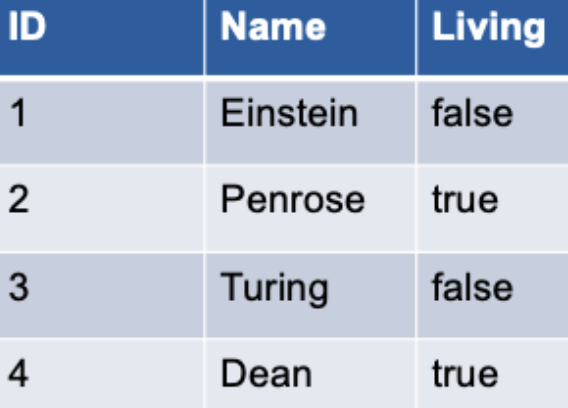
\includegraphics[width=0.6\textwidth]{Figures/FlatHomogeneous.png}
    \caption{Homogeneous flat Table}
\end{figure}
\end{minipage}

\begin{minipage}{0.55\textwidth}
\vspace{1\baselineskip}
\begin{lstlisting}[style=json,caption={JSON Code for a homogeneous and nested table.}]
{
    "ID":1,
    "Profession": "Physicist",
    "People": [
        {"Name": "Einstein", "Living" : false},
        {"Name": "Penrose", "Living" : true}
    ]
}
{
    "ID":2,
    "Profession": "Computer Scientist",
    "People": [
        {"Name": "Turing", "Living" : false},
        {"Name": "Dean", "Living" : true}
    ]
}
\end{lstlisting}
\end{minipage}
\hfill
\begin{minipage}{0.45\textwidth}
\begin{figure}[H]
    \centering
    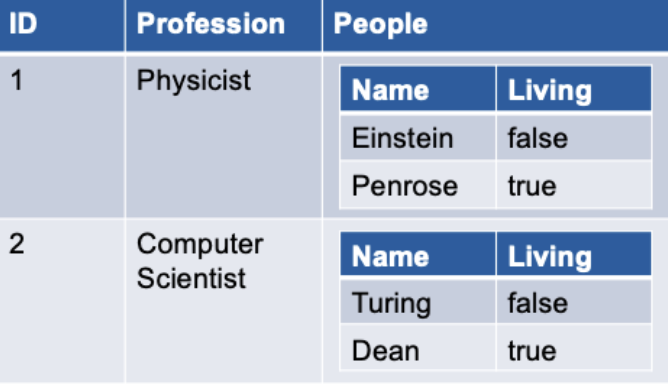
\includegraphics[width=0.9\textwidth]{Figures/NestedHomogeneous.png}
    \caption{Homogeneous nested Table}
\end{figure}
\end{minipage}


\begin{minipage}{0.55\textwidth}
\begin{lstlisting}[style=json,caption={JSON Code for a heterogeneous and flat table.}]
{
    "ID":1,
    "Name": "Einstein",
    "Living" : false,
    "Profession" : "Physicist"
}
{
    "ID":2,
    "Name": "Penrose",
    "Living" : true,
    "Profession" : "CS"
}
{
    "ID":3,
    "Name": "Turing"
}
{
    "ID":4,
    "Name": "Dean",
    "Living" : true
}
\end{lstlisting}
\end{minipage}
\hfill
\begin{minipage}{0.45\textwidth}
\begin{figure}[H]
    \centering
    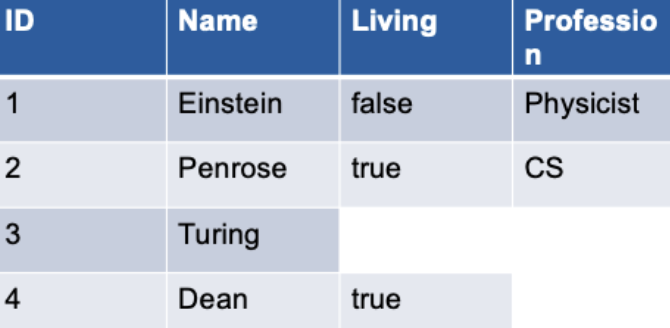
\includegraphics[width=0.9\textwidth]{Figures/FlatHeterogeneous.png}
    \caption{Heterogeneous flat Table}
\end{figure}
\end{minipage}


\begin{minipage}{0.55\textwidth}
\begin{lstlisting}[style=json,caption={JSON Code for a heterogeneous and nested table.}]
{
    "ID":1,
    "Profession": "Physicist",
    "People": [
        {"Name": "Einstein", "Living" : false},
        "Penrose"
    ]
} {
    "ID":2,
    "Profession": "Computer Scientist",
    "People": [
        {"Name": "Turing"},
        {"Name": "Dean", "Living" : true}
    ],
    "Comment": "They rock"
}
\end{lstlisting}
\end{minipage}
\hfill
\begin{minipage}{0.45\textwidth}
\begin{figure}[H]
    \centering
    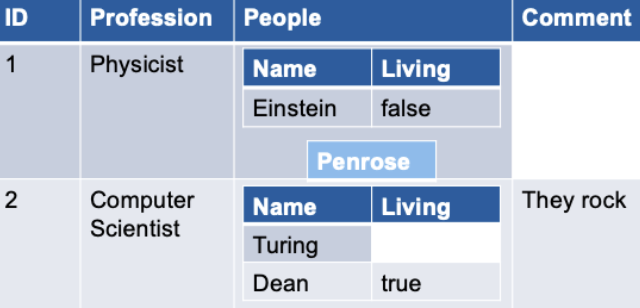
\includegraphics[width=0.9\textwidth]{Figures/NestedHeterogeneous.png}
    \caption{Heterogeneous nested Table}
\end{figure}
\end{minipage}


If the data is structured as a (valid) data frame, then there are many, many different formats that it can be stored in, and in a way that is much more efficient than JSON. These formats are highly optimized and typically stored in binary form, for example Parquet, Avro, Root, Google's protocol buffers, etc. If you see a JSON dataset that you are able to validate against a (e.g., JSound) schema that is "dataframe friendly", then you are highly encouraged to immediately build this schema, and convert the dataset to, say, Parquet. This gives you two immediate advantages:
\begin{itemize}
    \item space effciency: the file will be considerably smaller, meaning you can fit much more data even on your local laptop and it is also faster to transfer to and from the cloud to share with others.
    \item performance effciency: the smaller binary file will be much faster to read from disk when you write queries. In fact, many optimizers are able to skip entire sections of the data based on the query (projecting away a column, etc), making it even faster than it already was.
\end{itemize}
Generally, data formats can be classified along three dimensions:
\begin{itemize}
    \item whether they require validity against a data frame compatible schema (Parquet, protocol buffers, etc.) or not (JSON, XML, YAML, etc.).
    \item whether they allow for nestedness (Parquet, etc.) or not (CSV).
    \item whether they are textual (CSV, XML, JSON, etc.) or binary (Parquet, etc.), even though typically, formats that require a schema will be binary because of the “performance free lunch.”
\end{itemize}
